%%%%%%%%%%%%%%%%%%%%%%%%%%%%%%%%%%%%%%%%%%
\begin{frame}
    \frametitle{}
    \begin{center}
    { {\huge 第十二讲、矩阵表示}}
    \end{center}    
\end{frame}
%%%%%%%%%%%%%%%%%%%%%%%%%%%%%%%%%%%%%

\section{前情回顾}

\begin{frame}
    \frametitle{前情回顾}
    \begin{center}
        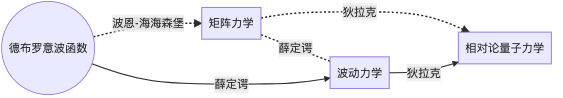
\includegraphics[width=0.9\textwidth]{figs/2021-12-06-16-22-39.png}\\   
    \end{center}
\end{frame}



\begin{frame}
    \frametitle{前情回顾}
    \begin{itemize}
        \item 波函数 : $$ \Psi(\vec{r},t)$$
        \item 薛定谔方程 :     
        \begin{equation*}
            i\hbar \frac{\partial }{\partial t} \Psi(\vec{r},t) = (\frac{\hbar^2}{2\mu} \nabla^2 +U(\vec{r})) \Psi(\vec{r},t)
        \end{equation*}
        \item 力学量算符 :
        $$\left\{ \begin{aligned}
            &\hat{\vec{r}} =\vec{r}  \\
            &\hat{\vec{p}} =-i\hbar(\dfrac{d}{d x}+ \dfrac{d}{d y} + \dfrac{d}{d z}) \\
            &\hat{F}=F(\hat{\vec{r}},\hat{\vec{p}}) \\
        \end{aligned} \right.$$
    \end{itemize}   
\end{frame} 

\section{表象理论}

\begin{frame} 
    \frametitle{}
    \begin{tcolorbox1}{定义:}
        \begin{itemize}
            \item 表象:波函数和力学量的具体表示形式,选择一个力学量本征函数系做为基就是选取一种表象
            \item 表象理论:研究量子力学各种表示形式以及它们之间的相互变换的理论。
            \item 矩阵表示:波函数在某个基上的展开系数构成矩阵 
        $$ \Psi(\vec{r},t)=\sum_n c_n(t) \psi_n(\vec{r})$$ 
        $$ \Psi\Leftrightarrow(c_1,c_2,\cdots)^T $$
        \end{itemize}   
    \end{tcolorbox1}
\end{frame} 

\section{波函数矩阵表示}
\begin{frame} 
    \frametitle{展开系数}    
    对于任意表象Q,若:\\
     本征分立谱: $\psi_n(\vec{r}) \to u_n(\vec{r})$, $c_n \to a_n $
        \begin{equation*}
            a_n(t)=(u_n(\vec{r}), \Psi(\vec{r},t)) 
        \end{equation*}  
    本征连续谱: $\psi_n(\vec{r}) \to u_q(\vec{r})$, $c_n \to a(q) $
        \begin{equation*}
            a(q,t)=(u_q(\vec{r}), \Psi(\vec{r},t)) 
        \end{equation*}  
\end{frame} 

\begin{frame} 
        \frametitle{1、波函数矩阵表示} 
        \begin{equation*}
            \begin{split} 
                \Psi(\vec{r},t)&=\sum_n a_n(t) u_n(\vec{r}) \\
                &=a_1(t) u_1+ a_2(t) u_2+\cdots+ a_n(t) u_n \\
                &=(u_1,u_2,\cdots,u_n) 
               \begin{pmatrix}
                    a_1(t)\\
                    a_2(t)\\
                    \cdots\\
                    a_n(t)
                \end{pmatrix} \\
                &= (u_1,u_2,\cdots,u_n) (a_1(t),a_2(t),\cdots, a_n(t))^T
            \end{split}  
        \end{equation*}  
        因此,有: $$   \Psi \Leftrightarrow (a_1(t),a_2(t),\cdots, a_n(t))^T \Leftrightarrow {\color{red}  \pmb {\Psi} } $$
\end{frame}

\begin{frame} 
    \frametitle{对比} 
    $$\begin{matrix}
      ~~  & \text{矢量空间} & \text{希尔伯特空间}\\ \vspace{0.6em}
      \text{基}  & \{\vec{e}_1,\vec{e}_2,\vec{e}_3\}  & \{ u_1,u_2,\cdots,u_n \}\\ \vspace{0.6em}
      \text{正交归一}  & \vec{e}_i \cdot \vec{e}_j=\delta_{ij} & ( u_m, u_n)= \delta_{mn}\\ \vspace{0.6em}
      \text{完备性}  & \vec{P}=\sum\limits_{i=1}^{3} x_i \vec{e}_i &  \Psi=\sum_n a_n(t) u_n \\  \vspace{0.6em}
      \text{投影}  & x_i= \vec{e}_i \cdot \vec{P}  & a_n(t)=( u_m, \Psi) \\ \vspace{0.6em}
      \text{矩阵}  & (x_1, x_2, x_3)^T & (a_1(t), a_2(t), \cdots, a_n(t))^T
      \end{matrix}
      $$
\end{frame}

\begin{frame} 
    \frametitle{实例} 
    \begin{tcolorbox2}{例1:}
        求动量本征态(平面波)在动量表象中的具体形式(矩阵表示)
    \end{tcolorbox2}
    \alert{解:} 动量的本征谱连续,采用公式\\
    $$a(q,t)=(u_q(\vec{r}), \Psi(\vec{r},t)) $$
    取 $$u_q(\vec{r})=\psi_{\vec{p}}(\vec{r})=\frac{1}{(2\pi\hbar)^{3/2}}e^{\frac{i}{\hbar}\vec{p}\cdot \vec{r}}, 
    \qquad \Psi(\vec{r},t))=\frac{1}{(2\pi \hbar)^{3/2}} e^{\frac{i}{\hbar}(\vec p\cdot \vec r -Et)} = 
    \psi_{\vec{p}'}e^{-\frac{i}{\hbar}Et}  $$
\end{frame}

\begin{frame} [allowframebreaks=]
    \frametitle{}
    \begin{equation*}
        \begin{split}
            a(q,t)&=(u_q(\vec{r}), \Psi(\vec{r},t)) \\
            a(p,t)&= (\psi_{\vec{p}}(\vec{r}), \psi_{\vec{p}'}e^{-\frac{i}{\hbar}Et})\\
            &= e^{-\frac{i}{\hbar}Et}(\psi_{\vec{p}}(\vec{r}), \psi_{\vec{p}'})\\
            &= e^{-\frac{i}{\hbar}Et}\delta(\vec{p}-\vec{p}')\\
        \end{split} 
    \end{equation*}
    \begin{tcolorbox}[colback=yellow!5,colframe=yellow!75!black,title=TIPS:]
        本征态在自身表象中的矩阵表示为$\delta$函数。
    \end{tcolorbox}
\end{frame} 

\begin{frame} [allowframebreaks=]
    \begin{tcolorbox2}{例2:}
        如下波函数是某体系的能量本征态\\
        $$ \psi_n(x)=\sqrt{\frac{2}{a}} \sin \frac{n\pi}{a}x, \qquad 0<x<a $$
        求基态(n=1)分别在动量和能量表象中的具体形式
    \end{tcolorbox2}
    \alert{解:} (1)动量的本征谱连续,采用公式\\
    \begin{equation*}
        \begin{split}
            a(q,t)&=(u_q(\vec{r}), \Psi(\vec{r},t)) \\
            a(p)&= (\psi_{p}(x), \psi_1(x))\\
            &= (\frac{1}{\sqrt{2\pi\hbar}}e^{\frac{i}{\hbar}px}, \sqrt{\frac{2}{a}} \sin \frac{\pi}{a}x)
        \end{split} 
    \end{equation*}

    \begin{equation*}
        \begin{split}
          ~~~~~~&= \frac{1}{\sqrt{2\pi\hbar}}\sqrt{\frac{2}{a}} (e^{\frac{i}{\hbar}px},  \sin \frac{\pi}{a}x)\\
            &= \frac{1}{\sqrt{2\pi\hbar}}\sqrt{\frac{2}{a}} \int_0 ^a e^{{\color{red}-}\frac{i}{\hbar}px}\sin \frac{\pi}{a}x) dx\\
            &=\sqrt{\frac{a\pi}{\hbar}} \frac{1+e^{\frac{i}{\hbar}pa}}{\pi^2-p^2a^2/\hbar^2}
        \end{split} 
    \end{equation*}

    (2)能量本征谱分立,采用公式\\
    \begin{equation*}
        \begin{split}
            a_n(t)&=(u_n(\vec{r}), \Psi(\vec{r},t)) \\
            a_{E_n}&=(\psi_n(x), \psi_1(x)) \\
            &=\delta_{1n} \\
        \end{split} 
    \end{equation*}  
\end{frame} 

\section{算符矩阵表示}
\begin{frame} [allowframebreaks=]
    \frametitle{2、算符矩阵表示}    
    算符有如下定义式:
    \begin{equation*}
        \varphi(\vec{r})=F\Psi(\vec{r}) 
    \end{equation*}  
    把两波函数在任意表象Q中展开 (基$u_n(\vec{r})$):\\
    \begin{equation*}
        \begin{split} 
         \sum_m b_m(t)u_m(\vec{r})&= F\sum_m a_m(t)u_m(\vec{r}) \\
         \sum_m b_m(t)u_m(\vec{r})&= \sum_m Fu_m(\vec{r})a_m(t) \\
         \sum_m b_m(t)u_n ^*(\vec{r}) u_m(\vec{r})&= \sum_m u_n ^*(\vec{r}) Fu_m(\vec{r})a_m(t) \\
         \sum_m b_m(t)(u_n (\vec{r}), u_m(\vec{r}))&= \sum_m (u_n (\vec{r}), Fu_m(\vec{r}))a_m(t) \\
         \sum_m b_m(t)\delta_{nm}&= \sum_m (u_n (\vec{r}), Fu_m(\vec{r}))a_m(t) \\
        \end{split}  
    \end{equation*} 
    \begin{equation*}
        \begin{split} 
         \sum_m b_m(t)\delta_{nm}&= \sum_m (u_n (\vec{r}), Fu_m(\vec{r}))a_m(t) \\
         b_n(t)&= \sum_m (u_n (\vec{r}), Fu_m(\vec{r}))a_m(t) \\
         b_n(t)&= \sum_m F_{nm} a_m(t) 
        \end{split}  
    \end{equation*} 
    取遍$n, m$, 得到如下矩阵形式\\
    $$\begin{pmatrix}
        b_1(t)\\
        b_2(t)\\
        \cdots \\
        b_n(t)
    \end{pmatrix}
    =
    \begin{pmatrix}
       F_{11} & F_{12} & \cdots & F_{1n} \\
       F_{21} & F_{22} & \cdots & F_{2n} \\
       \cdots & \cdots &  \cdots& \cdots\\
        F_{n1} & F_{n2} & \cdots & F_{nn} \\
    \end{pmatrix}
    \begin{pmatrix}
        a_1(t)\\
        a_2(t)\\
        \cdots \\
        a_n(t)
    \end{pmatrix}
    $$
    算符矩阵元公式: $$ F_{nm}=(u_n (\vec{r}), Fu_m(\vec{r})) $$
\end{frame} 

\section{算符矩阵表示的性质}
\begin{frame} 
    \frametitle{3、算符矩阵性质} 
    \begin{enumerate}
    \item  力学量算符的矩阵是厄密矩阵 
    \item  力学量算符的矩阵,对角元都是实数
    \item  力学量算符在自身表象是对角矩阵,对角元素就是算符的本征值
    \end{enumerate}
\end{frame}

\begin{frame} 
    \frametitle{定义} 
    \begin{tcolorbox1}{定义:}
        \begin{itemize}
        \item F的共轭矩阵: $F^{\dagger } =(F^*)^T$
        \item 厄密矩阵: $F= F^{\dagger }$
        \end{itemize}
    TIPS:厄密矩阵矩阵元特点 $$  F_{nm}^* = F_{mn}  $$
    \end{tcolorbox1}
\end{frame}

\begin{frame} 
    \frametitle{} 
    下列矩阵,哪些是厄密矩阵\\
    $$\begin{matrix}
        \begin{pmatrix}
            a & 0 & 0 & 0 \\
            0 & b & 0 & 0 \\
            0 & 0 & c & 0\\
            0 & 0 & 0 & 0 \\
         \end{pmatrix} 
         &  
         \begin{pmatrix}
            a & 1 & 0 & 0 \\
            2 & b & 0 & 0 \\
            0 & 0 & c & 0\\
            0 & 0 & 0 & 0 \\
         \end{pmatrix} 
         & 
         \begin{pmatrix}
            a & 1 & 0 & 0 \\
            1 & b & 0 & 0 \\
            0 & 0 & c & 0 \\
            0 & 0 & 0 & 0 \\
         \end{pmatrix} 
         \\ \vspace{0.6em}
         \begin{pmatrix}
            a & 1 & 0 & 0 \\
            -1 & b & 0 & 0 \\
            0 & 0 & c & 0 \\
            0 & 0 & 0 & 0 \\
         \end{pmatrix} 
         &     
        \begin{pmatrix}
            a & i & 0 & 0 \\
            i & b & 0 & 0 \\
            0 & 0 & c & 0 \\
            0 & 0 & 0 & 0 \\
        \end{pmatrix} 
         &   
         \begin{pmatrix}
            a & -i & 0 & 0 \\
            i & b & 0 & 0 \\
            0 & 0 & c & 0 \\
            0 & 0 & 0 & 0 \\
         \end{pmatrix} 
    \end{matrix}
        $$
\end{frame}


\begin{frame} [allowframebreaks=]
    \begin{tcolorbox1}{性质1:}
        试证明力学量算符的矩阵表示都是厄密矩阵
    \end{tcolorbox1}
    \alert{证明:} 
    \begin{equation*}
        \begin{split}
            F_{nm}&=(u_n (\vec{r}), Fu_m(\vec{r}))\\
            &=(Fu_n (\vec{r}), u_m(\vec{r}))\\
            &=(u_m(\vec{r}), Fu_n (\vec{r}))^*\\
            &=F_{mn}^*\\
        \end{split} 
    \end{equation*}
    证毕!
\end{frame}

\begin{frame} [allowframebreaks=]
    \begin{tcolorbox1}{性质2:}
        试证明力学量算符的矩阵表示,其对角元都是实数
    \end{tcolorbox1}
    \alert{证明:} 
    \begin{equation*}
        \begin{split}
            F_{nm}&=F_{mn}^*\\
            F_{nn}&=F_{nn}^*\\
        \end{split} 
    \end{equation*}
    即:对角元都是实数。 \\
    证毕!
\end{frame}

\begin{frame} [allowframebreaks=]
    \begin{tcolorbox1}{性质3:}
        试证明力学量算符的矩阵表示,在自身表象中是对角矩阵
    \end{tcolorbox1}
    \alert{证明:} 
    \begin{equation*}
        \begin{split}
            F_{nm}&=(u_n (\vec{r}), Fu_m(\vec{r}))\\
            &=(u_n (\vec{r}), f_nu_m(\vec{r}))\\
            &=f_n(u_n (\vec{r}), u_m(\vec{r}))\\
            &=f_n\delta_{mn}\\
        \end{split} 
    \end{equation*}
    即:(1)非对角元都是0,是对称阵。(2)对角元就是本征值\\
    证毕!
\end{frame}

\begin{frame} [allowframebreaks=]
    \begin{tcolorbox2}{对角化的物理意义}
        \begin{itemize}
            \item 力学量算符的表示一般不是对称阵(不在自身表象)
            \item 在数学上做矩阵对角化,使其成为对角阵 (在自身表象)
            \item 对角化完成从任意表象回到自身表象的过程
            \item 对角元就是本征值(解本征方程求本征值)
        \end{itemize}  
    \end{tcolorbox2}
\end{frame}

\begin{frame} 
    \frametitle{}
    \begin{tcolorbox2}{课堂作业:}
    取Q表象为动量表象,试求位置算符$\hat{x}$、动量算符$\hat{p}_x$ 的具体形式。
    \end{tcolorbox2}
\end{frame} 

\begin{frame} 
    \frametitle{}
    \begin{tcolorbox2}{课堂讨论}
    已知波函数取如下形式:$$\psi(x)=\frac{1}{\sqrt{2}}u_1(x)+\frac{1}{2}u_2(x)+\frac{1}{2}u_3(x)$$
    其系数矩阵为$$\begin{pmatrix}
            \frac{1}{\sqrt{2}}\\
            \frac{1}{2}\\
            \frac{1}{2}
            \end{pmatrix}$$
    \begin{enumerate}
        \item  此系数矩阵是波函数在位置表象的矩阵表示吗?
        \item  此系数矩阵是波函数在能量表象的矩阵表示的条件是什么?  
    \end{enumerate}
    \end{tcolorbox2}
\end{frame} 

\begin{frame} 
 THE END
\end{frame}

